\documentclass{article}
\usepackage{tikz}
\usetikzlibrary{graphs, positioning, quotes, shapes.geometric}

\begin{document}
	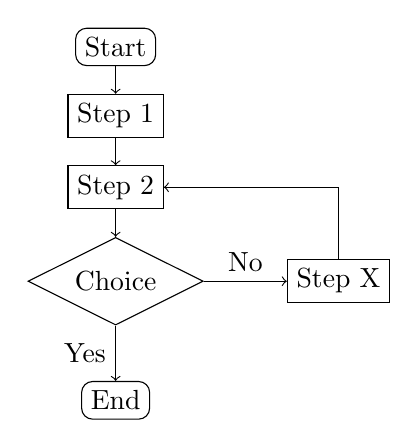
\begin{tikzpicture}[node distance=10pt]
		\node[draw, rounded corners]                        (start)   {Start};
		\node[draw, below=of start]                         (step 1)  {Step 1};
		\node[draw, below=of step 1]                        (step 2)  {Step 2};
		\node[draw, diamond, aspect=2, below=of step 2]     (choice)  {Choice};
		\node[draw, right=30pt of choice]                   (step x)  {Step X};
		\node[draw, rounded corners, below=20pt of choice]  (end)     {End};
		
		\graph{
			(start) -> (step 1) -> (step 2) -> (choice) ->["Yes"left] (end);
			(choice) ->["No"] (step x) ->[to path={|- (\tikztotarget)}] (step 2);
		};
	\end{tikzpicture}
\end{document}